\documentclass[11pt]{article}
\usepackage[review]{acl}

\usepackage{times}
\usepackage{latexsym}
\usepackage[T1]{fontenc}
\usepackage[utf8]{inputenc}
\usepackage{microtype}
\usepackage{inconsolata}
\usepackage{graphicx}
\usepackage{booktabs}
\usepackage{amsmath}
\usepackage{amsfonts}
\usepackage{multirow}
\usepackage{url}
\usepackage{tikz}
\usetikzlibrary{arrows.meta, positioning, fit, calc, backgrounds}

% Okabe-Ito Color Palette (Strict RGB)
\definecolor{oiBlue}{RGB}{0,114,178}
\definecolor{oiOrange}{RGB}{213,94,0}
\definecolor{oiGreen}{RGB}{0,158,115}
\definecolor{oiGray}{RGB}{110,110,110}

\emergencystretch=1.5em

\title{TRACER: Token-level Recursive Analysis, Control, and Evolutionary Refinement for Sequence Models}

\author{Anonymous Authors}

\begin{document}
\maketitle

\begin{abstract}
Recursive sequence models reapply a shared refinement operator to improve a prediction, yet most deployments run the same number of steps for every token. This spends work on already-correct tokens. Three questions remain: are the extra steps executed as counted, what changes inside the latent state, and does a step-size policy transfer? We find that high-confidence tokens keep their prediction across depths, which makes their refinement redundant and motivates early stopping. We present TRACER, a framework that measures transitions, halts on causal confidence, audits calls, and searches step sizes at fixed budget. Within TRACER, a one-shot 3{,}000-example development check shows that threshold halting on a frozen GRU executes 25.7\% of the deepest baseline's calls on two seeds and 51.8\% of the shallower $e_1$ baseline's calls on the third, with an exact-match change no larger than 0.20pp. Execution hooks verify that skipped refinements trigger no calls. Latent traces show that bounded gated states saturate after the first refinement, while unbounded accumulators keep growing. Across four architectures, 9 of 12 seeds are non-inferior or better and two are significantly worse. A 45-search study yields a median gain of 0.52pp, a single sample on the 192-example inner subset. A policy frozen on the GRU is non-inferior on 4 of 9 target seeds, and none is significantly worse. We release the framework and its audit protocol.
\end{abstract}

\section{Introduction}
\label{sec:intro}

A recursive sequence model reuses a shared refinement cell, so an early mistake can be repaired at a later step without adding parameters. Treating a Transformer as a recurrent update makes this view general \citep{katharopoulos2020transformers}, and looped Transformers show that repeating a fixed computation can implement algorithms a single pass cannot \citep{giannou2023looped,yang2024looped}. Multiple computational hops and relational recurrence make the same point for earlier architectures \citep{sukhbaatar2015memory,santoro2018relational}. Universal Transformers and recursive GRUs have shown that this extra computation improves reasoning and semantic parsing \citep{dehghani2019universal,graves2016adaptive}. The standard deployment fixes the number of passes in advance and runs every token through the same depth, even though conditional computation and token-level routing let a model spend different amounts on different inputs \citep{fedus2022switch,raposo2024mixture}. Tokens differ in difficulty: many are already correct after the first pass, and a few need the extra steps. On COGS \citep{kim2020cogs}, a benchmark where compositional generalization remains hard \citep{lake2018generalization,oren2020improving}, 87--91\% of examples keep their prediction across the first refinement, and only 5--9\% are repaired by it. The question is whether a token whose prediction is already stable needs the remaining refinement steps.

Accuracy at a fixed depth says little about the computation that produces it. Adjacent depths change the prediction on only a handful of tokens, and later passes can even flip a correct answer, a failure known as overthinking \citep{kaya2019shallowdeep}. That difference cannot tell us whether the model stored new information or merely rewrote the same state. Low-dimensional trajectories, fixed points, and update directions are the standard vocabulary for describing recurrent dynamics \citep{sussillo2013blackbox,vyas2020population,haviv2019memory}, and representation-similarity analysis warns that absolute coordinates from different systems are not directly comparable \citep{kriegeskorte2008rsa,kornblith2019cka}. We therefore record the latent state at every depth for four architectures and compare its norm, displacement, direction, and prediction change. In the bounded-state models the first refinement produces most of the state change, while later updates shrink to a fraction of that size, and this pattern holds only for seeds whose accuracy saturates after the first step. The unbounded states behave differently: the Transformer's updates stay nearly collinear across depths while its state norm grows steadily. This contrast raises a second question about the update itself. Iterative refinement in latent space can change an outcome at constant compute \citep{lee2020iterative,geng2021rewrite}, so the fixed refinement rule need not be the best one. A low-dimensional step size can be searched at a fixed evaluation budget, and evolutionary methods have long searched controller parameters without differentiating through a network \citep{stanley2002neat,such2017neuro}. Whether a policy frozen on one model still works in another remains a separate empirical question.

We present TRACER, a framework that treats recursion as something to measure before it is controlled. Its first component halts a token on confidence available before the refinement it gates; confidence-based inference already uses such readouts to adjust depth or abstain \citep{liu2020fastbert,xin2020deebert,geifman2017selective}. An active-subset executor with forward hooks confirms that skipped refinements are never computed. Its second component records latent trajectories across four architectures and reduces each trajectory to a norm, a displacement, and an update direction. These summaries describe change within a model across refinements and reveal where first-step gains saturate and where they do not. Its third component searches a five-parameter step-size policy under an equal budget of 336 evaluations and tests the frozen policy on held-out data and on three unseen architectures. Equal-budget comparison matters because the gain is small relative to seed variation, and non-inferiority testing supplies the right statistical frame for claiming that less compute does not cost accuracy \citep{docampobayon2025noninferiority,gu2023evaluation}. On COGS, halting preserves accuracy at a quarter of the deepest call count on most seeds, and the audited executor confirms that the saved calls are not executed. Single-sequence latency falls with the call count. The cross-architecture traces show two state regimes rather than one universal refinement dynamic. The evolutionary search returns a median gain of one inner-subset sample. The frozen policy is non-inferior on only part of the target seeds. We report these limits alongside the wins.

\section{Related Work}
\label{sec:related}

Recurrent computation has a long history in models that reuse a shared core. Neural programmer-interpreters made the core call subprograms and halt \citep{reed2016programmer}, while neural Turing machines paired a finite controller with an external memory \citep{graves2014neural}. End-to-end memory networks repeated an attention module over several hops \citep{sukhbaatar2015memory}, and relational recurrent networks added point-product attention to the recurrent state \citep{santoro2018relational}. Transformer-XL carried state across segments \citep{dai2019transformerxl}, the recurrent memory transformer added explicit memory tokens \citep{bulatov2022recurrent}, and RWKV reformulated linear attention as a recurrent update \citep{peng2023rwkv}. Retentive networks connect recurrence and attention as three equivalent computational views \citep{sun2023retentive}. These lines of work established that repeated computation can improve a prediction without a proportional increase in parameters. Most evaluations still stop at final accuracy: they report what deeper recursion achieves, not how much each individual refinement contributes, how often it changes a decision, or whether the latent state changes at all.

Dynamic depth has been studied from several angles. BranchyNet placed early classifiers at intermediate layers \citep{teerapittayanon2016branchynet}, and multi-scale dense networks made every layer an exit point \citep{huang2018multiscale}. Spatially adaptive computation time allocated layers per image position \citep{figurnov2017spatially}, which is the visual analogue of token-level compute allocation. Bolukbasi et al. learned per-layer exits from a global objective \citep{bolukbasi2017adaptive}, and FastBERT and DeeBERT applied confidence-gated exits to pretrained language models \citep{liu2020fastbert,xin2020deebert}. PATience-based exiting used prediction stability rather than a single probability \citep{zhou2020patience}, and mixture-of-depths routed tokens through different layer counts \citep{raposo2024mixture}. Switch Transformers scaled conditional computation by activating only part of the parameters per token \citep{fedus2022switch}. These methods train the exit decision jointly with the network and typically report savings through the depth or step count their controller selects. A frozen model offers no such gate to train, so a threshold must read signals already present at the decision point. The quality of those signals is itself a studied question \citep{jiang2018trust,tian2023calibration}. Savings are real only if the decoder omits the gated refinement, which calls for counting executed calls instead of inferring depth.

Iterative refinement revises an initial output in successive passes. Deterministic non-autoregressive modeling framed each pass as a denoising step \citep{lee2018deterministic}, and latent refinement moved the update into a low-dimensional continuous space \citep{lee2020iterative}. MR-P let a decoder stop when its refinement converged \citep{cheng2022mrp}, and a recent empirical study measured redundant rewrites and confidence changes across refinement steps \citep{xiao2025empirical}. Work on semantic parsing showed that structured rewrites can repair span-level errors that a single pass misses \citep{geng2021rewrite}. In all of these, the number of passes is either fixed or chosen by a trained controller; the present study keeps the passes fixed and asks whether the update applied at each one can be rescaled under a frozen model.

Trajectory readouts give a vocabulary for what a refinement changes. Low-dimensional dynamics in high-dimensional recurrent networks are described by fixed points and state geometry \citep{sussillo2013blackbox,vyas2020population}, with state velocity defining how far a trajectory moves in one step \citep{haviv2019memory}. Dynamical similarity analysis cautions that equivalent computations need not share a geometry \citep{ostrow2023dsa}, and structured state-space models define states whose scale and meaning differ from a gated recurrent state \citep{gu2022s4,gu2023mamba}. Visualizing individual units showed why the LSTM cell state and hidden state must be read apart \citep{karpathy2015rnn}, and geometry studies analyzed representation dynamics layer by layer \citep{horoi2020geometry}. These observations motivate within-model summaries of norm, displacement, and direction, and they rule out ranking architectures by absolute state norm.

Derivative-free search supplies the third component. Genetic algorithms remain a standard black-box optimizer \citep{whitley1994tutorial}, differential evolution uses difference vectors between population members as perturbations \citep{storn1997de,das2011survey}, and CMA-ES adapts a covariance matrix to the search landscape \citep{hansen2001cma,hansen2003cma}. Surveys of derivative-free optimization compare these methods under a common function-value budget \citep{rios2013df}, and evolutionary approaches have searched network topologies and controllers since NEAT \citep{stanley2002neat,such2017neuro}. Here the search adjusts only the step size of an executed refinement; weights stay fixed, and the budget is matched across algorithms. We ask how much a five-parameter update policy gains at constant depth, whether that gain survives on held-out data, and whether it carries to another architecture.

\section{Method}
\label{sec:method}

We begin with a frozen recursive sequence model that produces four decoding depths, from $e_0$ to $e_3$. The base step reads the source memory, the previous token, and the previous hidden state to produce $z^{(0)}$. A shared refinement cell maps $z^{(k)}$ to $z^{(k+1)}$ using the previous token, the base attention context, and a soft embedding of the current prediction. In the checkpoints used below, training applies multi-depth supervision at all four depths with weights $(0.1,0.2,0.3,0.4)$, and a single output head is shared across them. Every later component keeps these parameters fixed and operates on the same four-depth rollout.

\begin{figure}[t]
\centering
\resizebox{\columnwidth}{!}{%
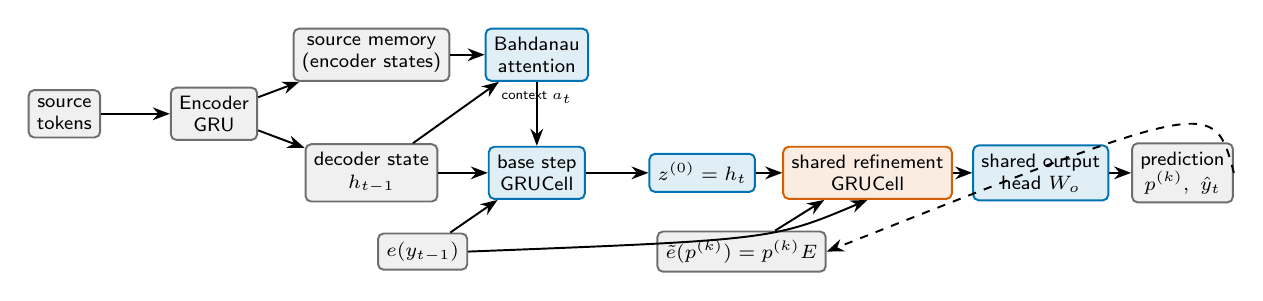
\begin{tikzpicture}[font=\sffamily\scriptsize, >=Stealth, line width=0.7pt,
  b/.style={draw, rounded corners=2pt, align=center, inner sep=3pt},
  g/.style={b, draw=oiGray, fill=oiGray!10},
  u/.style={b, draw=oiBlue, fill=oiBlue!12},
  o/.style={b, draw=oiOrange, fill=oiOrange!12}]
\node[g] (src) at (0,0) {source\\tokens};
\node[g] (enc) at (1.9,0) {Encoder\\GRU};
\node[g] (mem) at (3.9,0.75) {source memory\\(encoder states)};
\node[g] (st) at (3.9,-0.75) {decoder state\\$h_{t-1}$};
\node[u] (att) at (6.0,0.75) {Bahdanau\\attention};
\node[u] (base) at (6.0,-0.75) {base step\\GRUCell};
\node[g] (emb) at (4.55,-1.75) {$e(y_{t-1})$};
\node[u] (z0) at (8.1,-0.75) {$z^{(0)}=h_t$};
\node[o] (ref) at (10.2,-0.75) {shared refinement\\GRUCell};
\node[g] (soft) at (8.6,-1.75) {$\tilde e(p^{(k)})=p^{(k)}E$};
\node[u] (out) at (12.4,-0.75) {shared output\\head $W_o$};
\node[g] (pred) at (14.2,-0.75) {prediction\\$p^{(k)},\ \hat y_t$};
\draw[->] (src) -- (enc);
\draw[->] (enc) -- (mem); \draw[->] (enc) -- (st);
\draw[->] (mem) -- (att); \draw[->] (st) -- (att);
\draw[->] (att) -- node[above,font=\sffamily\tiny] {context $a_t$} (base);
\draw[->] (emb) -- (base); \draw[->] (st) -- (base);
\draw[->] (base) -- (z0); \draw[->] (z0) -- (ref);
\draw[->] (soft) -- (ref); \draw[->] (emb.east) .. controls (9.0,-1.6) .. (ref.south);
\draw[->] (ref) -- (out); \draw[->] (out) -- (pred);
\draw[->,dashed] (pred.east) .. controls (14.6,0.2) .. (soft.east);
\end{tikzpicture}%
}
\caption{Recursive encoder--decoder architecture reproduced from the implemented model. The encoder produces a source memory and an initial decoder state. A base \textsc{GRUCell} emits $z^{(0)}$ from the previous token embedding and the attention context. A single refinement \textsc{GRUCell}, shared across all depths, reads the previous token embedding, the same context, and a soft embedding of the current prediction. One output head is shared across depths.}
\label{fig:arch}
\end{figure}

On this rollout, we first measure what the extra depths buy. For every token, we compare its predictions at two adjacent depths and assign one of four outcomes. A wrong prediction that becomes correct is a repair, and a correct one that becomes wrong is harm. When the prediction is unchanged, we call it preserve if it was correct and unresolved if it was wrong. This separation matters because a single-depth accuracy score folds together tokens that refinement fixed and tokens that refinement broke.

\begin{figure}[t]
\centering
\resizebox{\columnwidth}{!}{%
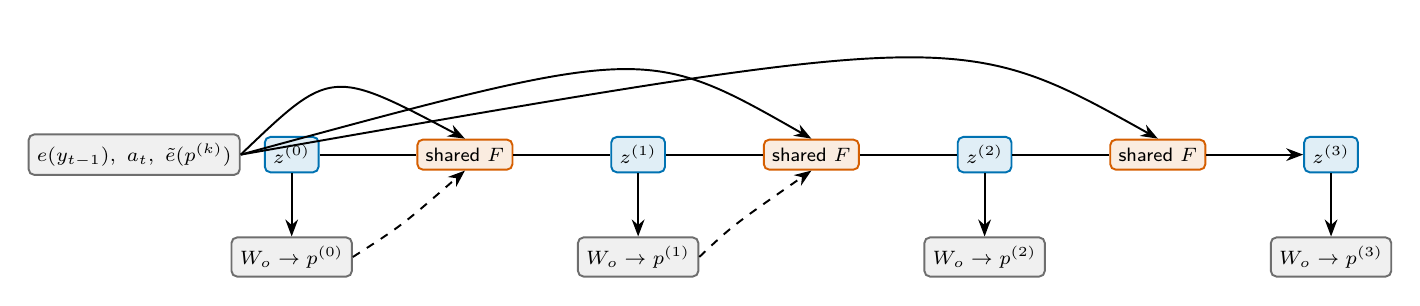
\begin{tikzpicture}[font=\sffamily\scriptsize, >=Stealth, line width=0.7pt,
  b/.style={draw, rounded corners=2pt, align=center, inner sep=3pt},
  u/.style={b, draw=oiBlue, fill=oiBlue!12},
  g/.style={b, draw=oiGray, fill=oiGray!10},
  o/.style={b, draw=oiOrange, fill=oiOrange!12}]
\node[g] (inp) at (0,0) {$e(y_{t-1}),\ a_t,\ \tilde e(p^{(k)})$};
\node[u] (z0) at (2.0,0) {$z^{(0)}$};
\node[o] (r0) at (4.2,0) {shared $F$};
\node[u] (z1) at (6.4,0) {$z^{(1)}$};
\node[o] (r1) at (8.6,0) {shared $F$};
\node[u] (z2) at (10.8,0) {$z^{(2)}$};
\node[o] (r2) at (13.0,0) {shared $F$};
\node[u] (z3) at (15.2,0) {$z^{(3)}$};
\node[g] (o0) at (2.0,-1.3) {$W_o \to p^{(0)}$};
\node[g] (o1) at (6.4,-1.3) {$W_o \to p^{(1)}$};
\node[g] (o2) at (10.8,-1.3) {$W_o \to p^{(2)}$};
\node[g] (o3) at (15.2,-1.3) {$W_o \to p^{(3)}$};
\draw[->] (z0) -- (r0) -- (z1) -- (r1) -- (z2) -- (r2) -- (z3);
\draw[->] (inp.east) .. controls (2.5,1.1) .. (r0.north);
\draw[->] (inp.east) .. controls (6.5,1.4) .. (r1.north);
\draw[->] (inp.east) .. controls (10.5,1.6) .. (r2.north);
\draw[->] (z0) -- (o0); \draw[->] (z1) -- (o1); \draw[->] (z2) -- (o2); \draw[->] (z3) -- (o3);
\draw[->,dashed] (o0.east) .. controls (3.4,-0.9) .. (r0.south);
\draw[->,dashed] (o1.east) .. controls (7.6,-0.9) .. (r1.south);
\end{tikzpicture}%
}
\caption{Recursive refinement at one output position. The base step produces $z^{(0)}$. The same refinement operator $F$ maps $z^{(k)}$ to $z^{(k+1)}$ using the previous token embedding, the base attention context, and the soft embedding $p^{(k)}E$ of the current prediction. The shared output head emits a distribution at every depth; no new parameters are added as depth grows.}
\label{fig:refine}
\end{figure}

The transitions above are token-specific, so we decide for each token whether to spend the extra computation. Causal halting makes this decision at two points on the rollout: after the base step and again after the first refinement. At each point we compare the top-1 probability of the current prediction with a fixed threshold. A token stops when the probability exceeds that threshold; the two thresholds are $0.85$ and $0.90$ for every model and seed. Each decision uses only signals computed before the refinement it gates, so a stopped token never reads the computation it has chosen to skip. A token that passes both gates continues to $e_3$.

\begin{figure}[t]
\centering
\resizebox{\columnwidth}{!}{%
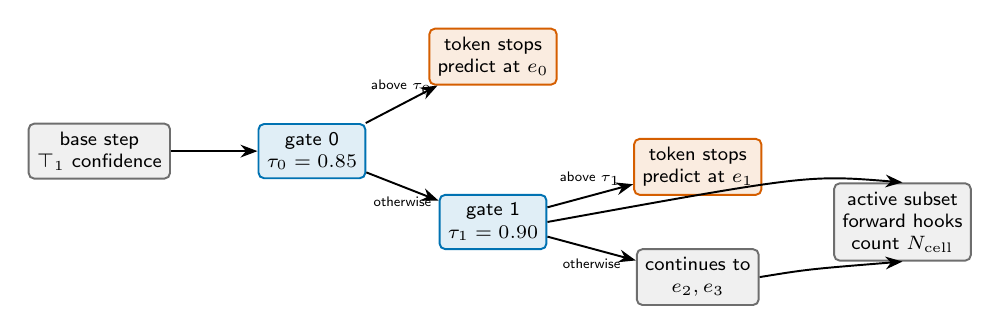
\begin{tikzpicture}[font=\sffamily\scriptsize, >=Stealth, line width=0.7pt,
  b/.style={draw, rounded corners=2pt, align=center, inner sep=3pt},
  u/.style={b, draw=oiBlue, fill=oiBlue!12},
  g/.style={b, draw=oiGray, fill=oiGray!10},
  r/.style={b, draw=oiOrange, fill=oiOrange!12}]
\node[g] (base) at (0,0) {base step\\$\top_1$ confidence};
\node[u] (g0) at (2.7,0) {gate 0\\$\tau_0=0.85$};
\node[r] (s0) at (5.0,1.2) {token stops\\predict at $e_0$};
\node[u] (g1) at (5.0,-0.9) {gate 1\\$\tau_1=0.90$};
\node[r] (s1) at (7.6,-0.2) {token stops\\predict at $e_1$};
\node[g] (deep) at (7.6,-1.6) {continues to\\$e_2,e_3$};
\node[g] (audit) at (10.2,-0.9) {active subset\\
forward hooks\\count $N_{\mathrm{cell}}$};
\draw[->] (base) -- (g0);
\draw[->] (g0) -- node[above,font=\sffamily\tiny] {above $\tau_0$} (s0);
\draw[->] (g0) -- node[below,font=\sffamily\tiny] {otherwise} (g1);
\draw[->] (g1) -- node[above,font=\sffamily\tiny] {above $\tau_1$} (s1);
\draw[->] (g1) -- node[below,font=\sffamily\tiny] {otherwise} (deep);
\draw[->] (g1.east) .. controls (9.0,-0.3) .. (audit.north);
\draw[->] (deep.east) .. controls (9.0,-1.5) .. (audit.south);
\end{tikzpicture}%
}
\caption{Causal token-level halting. Each gate reads only signals computed before the refinement it controls, so a stopped token never consults the computation it skips. The predicted exit depth is not the same quantity as executed work: the active-subset executor runs a cell only on continuing rows, and forward hooks verify the intercepted call count against $N_{\mathrm{cell}}$.}
\label{fig:halt}
\end{figure}

Predicted exit depth and executed calls are different quantities. To measure the latter, the executor gathers the active rows before each base call and the continuing rows before each refinement call. It scatters their outputs back into the batch, so finished and stopped rows never enter a call. We define $N_{\mathrm{cell}}$ as the calls the executor makes: one base call per active row plus one call per refinement that row executes. Forward hooks on the decoder and refinement cells record the input row count of every call. When these hook counts match $N_{\mathrm{cell}}$, the drop in counted calls reflects computation the executor really did not perform.

Halting decides when to stop, not what a refinement does to the state. We record the latent vector at every generated position and depth, together with the predictive distribution and the predicted token, giving a trajectory $z^{(0)},\dots,z^{(3)}$ per token. Recording runs under free-running greedy decoding on a fixed group-balanced source sample, applied to each model in turn; teacher forcing is reserved for training-time diagnostics and is not used for these trajectories.

From each trajectory we compute six summaries: the normalized state norm $\lVert z_k\rVert/\sqrt d$, the update norm, the relative update, the cosine between consecutive updates, the total displacement from $z^{(0)}$, and the rate at which the predicted token changes across depths. Token-level values are averaged within each example first, then resampled by a group-cluster bootstrap for a 95\% interval. We keep LSTM's hidden and cell states separate, and Mamba's decoder latent separate from its internal SSM state; Mamba is a single-seed descriptive probe and is excluded from the main table.

The refinement rule itself need not be the best update. At a fixed depth we rescale each step as $z^{(k+1)}=z^{(k)}+\alpha^{(k)}\Delta z^{(k)}$, with $\alpha^{(k)}=\sigma(w_0+w_1\tilde H+w_2\tilde D+w_3\tilde A+w_4\,k/K)$: an intercept plus four causally available features, prediction entropy $H$, update magnitude $D$, update direction $A$, and depth $k/K$. The search changes only these five coefficients; model weights and the number of refinement steps stay fixed, so any accuracy change is a latent-dynamics effect at constant compute.

\begin{figure}[t]
\centering
\resizebox{\columnwidth}{!}{%
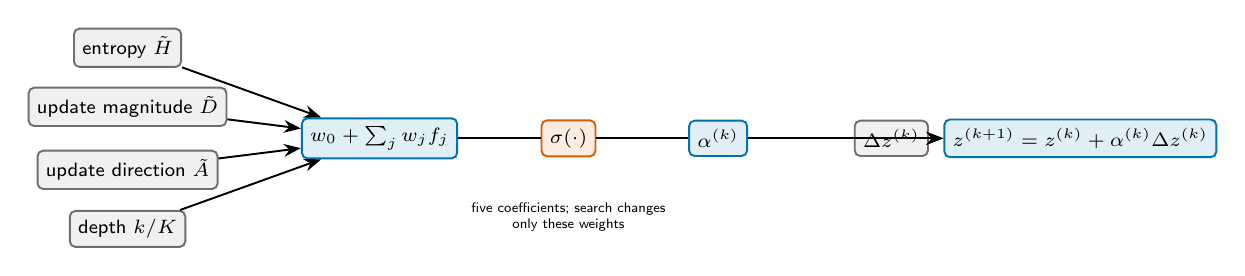
\begin{tikzpicture}[font=\sffamily\scriptsize, >=Stealth, line width=0.7pt,
  b/.style={draw, rounded corners=2pt, align=center, inner sep=3pt},
  g/.style={b, draw=oiGray, fill=oiGray!10},
  u/.style={b, draw=oiBlue, fill=oiBlue!12},
  o/.style={b, draw=oiOrange, fill=oiOrange!12}]
\node[g] (H) at (0,1.15) {entropy $\tilde H$};
\node[g] (D) at (0,0.4) {update magnitude $\tilde D$};
\node[g] (A) at (0,-0.4) {update direction $\tilde A$};
\node[g] (k) at (0,-1.15) {depth $k/K$};
\node[u] (lin) at (3.2,0) {$w_0+\sum_j w_j f_j$};
\node[o] (sig) at (5.6,0) {$\sigma(\cdot)$};
\node[u] (a) at (7.5,0) {$\alpha^{(k)}$};
\node[g] (dz) at (9.7,0) {$\Delta z^{(k)}$};
\node[u] (eq) at (12.1,0) {$z^{(k+1)}=z^{(k)}+\alpha^{(k)}\Delta z^{(k)}$};
\draw[->] (H) -- (lin); \draw[->] (D) -- (lin); \draw[->] (A) -- (lin); \draw[->] (k) -- (lin);
\draw[->] (lin) -- (sig) -- (a) -- (eq); \draw[->] (dz) -- (eq);
\node[font=\sffamily\tiny,align=center] at (5.6,-1.0) {five coefficients; search changes\\only these weights};
\end{tikzpicture}%
}
\caption{Evolutionary latent step-size control. Four causally available features and an intercept form a five-parameter policy. A sigmoid maps them to $\alpha^{(k)}$, which rescales the refinement displacement at fixed depth. Model weights and the number of refinement steps are unchanged, so any accuracy difference isolates the update rule.}
\label{fig:alpha}
\end{figure}

Five algorithms search the same policy under a common budget of 336 evaluations: random search, a genetic algorithm, a mutation-guided variant, differential evolution, and sep-CMA-ES. For each model seed we take the best policy on the inner folds, freeze its weights and feature-normalization statistics, and confirm it once on a 640-sample outer fold. We then apply that frozen policy unchanged to Vanilla RNN, LSTM, and Transformer with no further search, and report the seeds that are non-inferior and those that are not.

\begin{figure}[t]
\centering
\resizebox{\linewidth}{!}{%
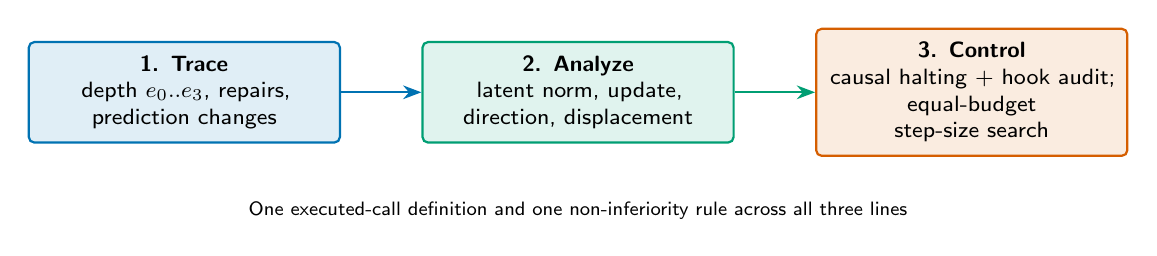
\begin{tikzpicture}[
  font=\sffamily\fontsize{8pt}{9.6pt}\selectfont,
  >=Stealth, line width=0.8pt,
  box/.style={draw, rounded corners=2pt, inner sep=5pt, text width=3.6cm, align=center},
  blue/.style={box, draw=oiBlue, fill=oiBlue!12},
  green/.style={box, draw=oiGreen, fill=oiGreen!12},
  orange/.style={box, draw=oiOrange, fill=oiOrange!12}
]
\node[blue] (a) at (0,2.2) {\textbf{1. Trace}\\ depth $e_0..e_3$, repairs,\\ prediction changes};
\node[green] (b) at (5.0,2.2) {\textbf{2. Analyze}\\ latent norm, update,\\ direction, displacement};
\node[orange] (c) at (10.0,2.2) {\textbf{3. Control}\\ causal halting + hook audit;\\ equal-budget step-size search};
\draw[->,draw=oiBlue] (a) -- (b);
\draw[->,draw=oiGreen] (b) -- (c);
\node[align=center,font=\sffamily\fontsize{7.4pt}{9pt}\selectfont] at (5.0,0.7)
  {One executed-call definition and one non-inferiority rule across all three lines};
\end{tikzpicture}%
}
\caption{TRACER: measure recursive computation, analyze the latent trajectory, then control execution and updates. Each line is evaluated with the same frozen checkpoints and call-counting rule.}
\label{fig:framework}
\end{figure}

\section{Experiments}
\label{sec:exp}

We evaluate TRACER on COGS, a semantic parsing benchmark that maps natural language to logical forms, and hold one setup fixed across three questions: what the extra steps execute, what they change in the latent state, and whether a step-size policy transfers. One executed-call counter and one non-inferiority rule decide all three.

\subsection{Dataset}
COGS tests compositional generalization by mapping natural language to logical forms \citep{kim2020cogs}. The broader difficulty of systematic generalization \citep{keysers2020measuring,furrer2020compositional} has driven structured parsers \citep{herzig2021span,shaw2021compositional} and disentangled models \citep{zheng2022disentangled}, yet scaling alone does not remove it \citep{qiu2022evaluating,li2023slog}, and COGS remains a standard benchmark \citep{weissenhorn2022compositional}. COGS contains 24{,}155 training, 3{,}000 development, 3{,}000 test, and 21{,}000 generalization examples; the official test and generalization splits remain sealed and were never read. Cross-architecture evaluation and latent analysis share one fixed, group-balanced sample of 256 training examples across all models and seeds. Optimizer search runs on an inner subset fixed before search, and each policy selected there is confirmed once on an outer fold of about 640 training examples. A final check applies only the frozen threshold policy to the official 3{,}000-example development set, evaluated once and marked used thereafter.

\subsection{Experimental Environment}
All experiments use the same local CPU workstation; wall-clock timing fixes the thread count at two. GRU, Vanilla RNN, LSTM, and Transformer are each trained at three seeds, alongside a single-seed Mamba-1-Tiny boundary probe (Table~\ref{tab:models}). We train with Adam at $10^{-3}$, batch size 32, and 15 epochs, using 64-dimensional embeddings and 128-dimensional hidden states for the GRU-family models; the recursive Transformer instead uses a 128-dimensional width. Refinement runs up to three steps under multi-depth supervision weighted $(0.1,0.2,0.3,0.4)$ over $e_0$--$e_3$, with model seeds 0, 1, and 2. Five algorithms search at three optimizer seeds each, with 336 candidate evaluations per run. Non-inferiority holds when the lower bound of a 95\% group-cluster bootstrap interval on $\Delta$EM reaches $-0.5$pp or above; the point estimate alone does not decide it.

\begin{table}[t]
\centering
\footnotesize
\begin{tabular}{@{}llc@{}}
\toprule
Model & Core structure & Params \\
\midrule
GRU & GRUCell + Bahdanau attn & 560K \\
Vanilla RNN & RNNCell + dot attn & 343K \\
LSTM & LSTMCell + dot attn & 689K \\
Transformer & recursive, width 128 & 799K \\
Mamba & Mamba-1 S6, 64 & 149K \\
\bottomrule
\end{tabular}
\caption{Architectures. Mamba is a single-seed boundary probe.}
\label{tab:models}
\end{table}

\subsection{Experimental Design}
TRACER runs three lines of study in a fixed order, each posed by the previous one. We first measure what each recursive depth contributes and use that picture to design a causal stopping rule. We then record latent trajectories to ask what the extra steps change in the state. Finally we fix the depth, search a step-size policy, and test it on held-out data and on unseen architectures. The three lines share the frozen checkpoints and one definition of an executed call; the two diagnostic lines read a common 256-example manifest, while the search uses its own inner and outer folds.

The depth study trains three seeds per architecture and decodes the same 256 group-balanced examples at $e_0$ through $e_3$. For each adjacent pair we count repair, harm, preserve, and unresolved outcomes. Plotting accuracy against depth shows where gains saturate and where refinement keeps changing predictions after the model has settled.

The halting study places two gates on that rollout, after the base step and after the first refinement, at fixed thresholds $0.85$ and $0.90$. We compare the halted decode with forced $e_3$ and with each seed's best fixed depth, reporting EM, paired bootstrap intervals, and $N_{\mathrm{cell}}$. An active-subset executor with forward hooks checks that the skipped refinements trigger no calls. We further time batch sizes 1, 4, 8, and 32 to see how much of the call saving survives as wall-clock time; Transformer uses its own per-sample decoder and is reported separately.

The ablations separate two questions. Under the shared 256-sample protocol we contrast the fixed threshold with forced-stop ($e_0$) and forced-continue ($e_3$) controls, and the hook counts verify that the omitted refinements are not executed; this rules out an accounting artifact. On a separate single-architecture GRU setup (fold-4, 645 examples per seed), a descriptive sweep over threshold pairs and a comparison of top-1 with margin and entropy readouts place the frozen threshold on a flat non-inferior plateau; neither sweep reselects the policy.

Halting changes which steps run, not what a step does to the state. The latent study uses the 256-sample manifest and records $e_0$--$e_3$ trajectories for the four main architectures at three seeds each. Each token contributes a state vector, quantities derived from the predictive distribution, and its prediction. We compute six summaries per depth, average them within each example, and resample groups for confidence intervals. LSTM hidden and cell states are kept apart.

We plot the trajectories of all four architectures in shared panels and check whether the first-refinement pattern holds across seeds. Two regimes are kept separate: bounded gated states (GRU, Vanilla RNN, LSTM hidden state) and growing unbounded accumulators (LSTM cell state and Transformer). These are descriptive comparisons, not controlled cell ablations, because attention type and parameter count also differ. The single-seed Mamba probe contributes a 64-sample description of its decoder latent and internal SSM state, which stays out of the four-architecture statistics.

The search fixes the recursive depth and the model weights. A five-parameter policy scales each refinement, and five algorithms (random search, a genetic algorithm, a mutation-guided variant, differential evolution, and sep-CMA-ES) search it at three optimizer seeds per model seed, with 336 evaluations per run. The baseline is the original update with $\alpha\equiv1$, so any gain isolates the step-size effect at constant depth.

We ablate the policy inputs in three groups: the depth index, prediction entropy, and latent-dynamics features (update magnitude and direction). We also record the selected $\alpha$ at each depth and the tokens whose predictions change, in order to ask whether the gain comes from a depth schedule or from content-dependent updates. The ablations do not uniquely favor either account.

The best inner policy is frozen and confirmed once on a 640-example outer fold. That single GRU policy and its feature-normalization statistics are then applied unchanged to all three seeds of Vanilla RNN, LSTM, and Transformer, with no re-search. Each target seed is classified by the non-inferiority bound, and seeds that meet neither non-inferiority nor a significant loss are reported as inconclusive.

The three lines combine into one account. The latent curves show why halting is safe where depth one already saturates, the call counts say what the saving consists of, and the step-size search bounds what a frozen update policy gains before transfer fails to hold. We report the negative cases alongside the positive ones.


\section{Results and Analysis}
\label{sec:results}

Three questions organize this section: are the counted extra steps executed, what changes inside the latent state, and does a tuned update rule survive transfer? Every claim below is backed by a table or figure computed from the released result files. Negative and inconclusive cases are reported in the same passages as the positive ones.

\textbf{Recursive computation and causal halting.} \begin{figure}[t]
\centering
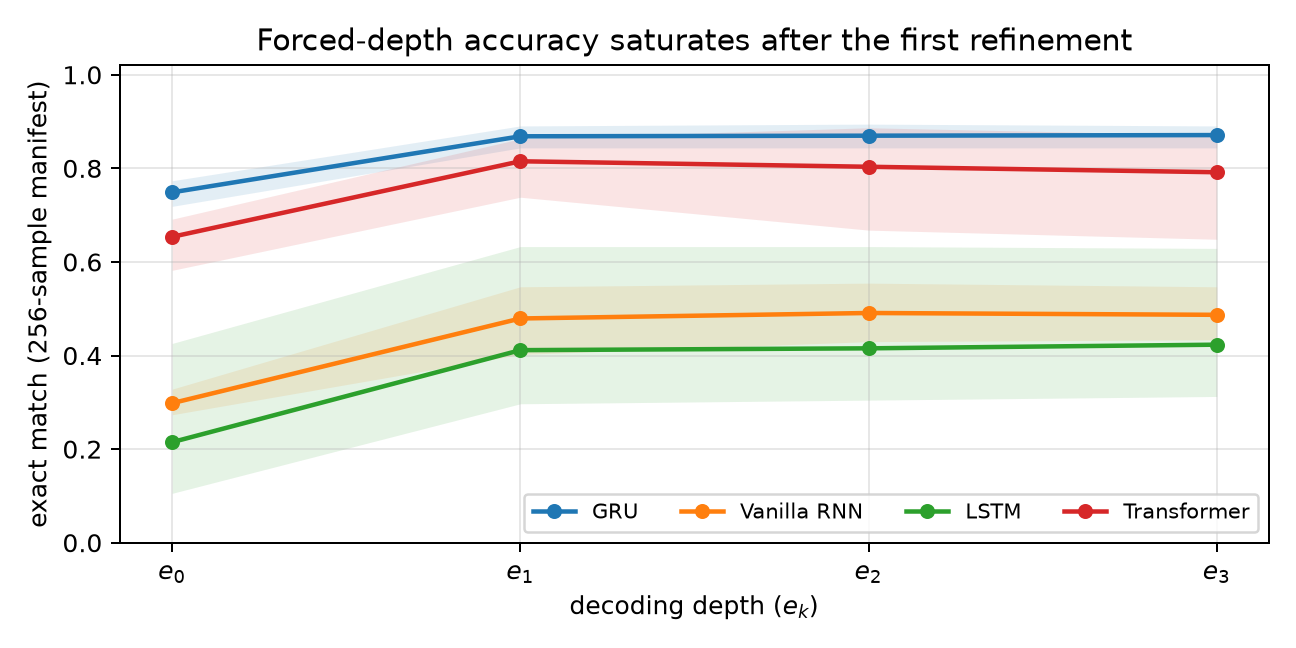
\includegraphics[width=\columnwidth]{figures/fig_depth.png}
\caption{Forced exact match by depth for four architectures. Lines are seed means; shaded bands span three seeds (256 group-balanced examples).}
\label{fig:depth}
\end{figure} \begin{table}[t]
\centering
\footnotesize
\begin{tabular}{lcccc}
\toprule
Architecture & $e_0$ & $e_1$ & $e_2$ & $e_3$ \\
\midrule
GRU & $0.749$ & $0.868$ & $0.870$ & $0.871$ \\
Vanilla RNN & $0.298$ & $0.479$ & $0.491$ & $0.487$ \\
LSTM & $0.215$ & $0.411$ & $0.415$ & $0.423$ \\
Transformer & $0.654$ & $0.815$ & $0.803$ & $0.792$ \\
\bottomrule
\end{tabular}
\caption{Forced exact match by depth, seed-averaged over three seeds per architecture (256 group-balanced examples).}
\label{tab:depth}
\end{table} Figure~\ref{fig:depth} and Table~\ref{tab:depth} show what depth adds. Forced exact match rises sharply from $e_0$ to $e_1$ and then flattens: within each architecture, the first refinement delivers 94--98\% of the accuracy gain reached at $e_3$ on GRU, Vanilla RNN, and LSTM. The three-seed $e_3$ scores are 0.879/0.844/0.891 (GRU), 0.434/0.547/0.480 (Vanilla RNN), 0.629/0.312/0.328 (LSTM), and 0.871/0.648/0.855 (Transformer). Transformer also peaks by $e_1$ in accuracy, but its latent state keeps changing, a difference taken up in the second line of results.

\begin{figure}[t]
\centering
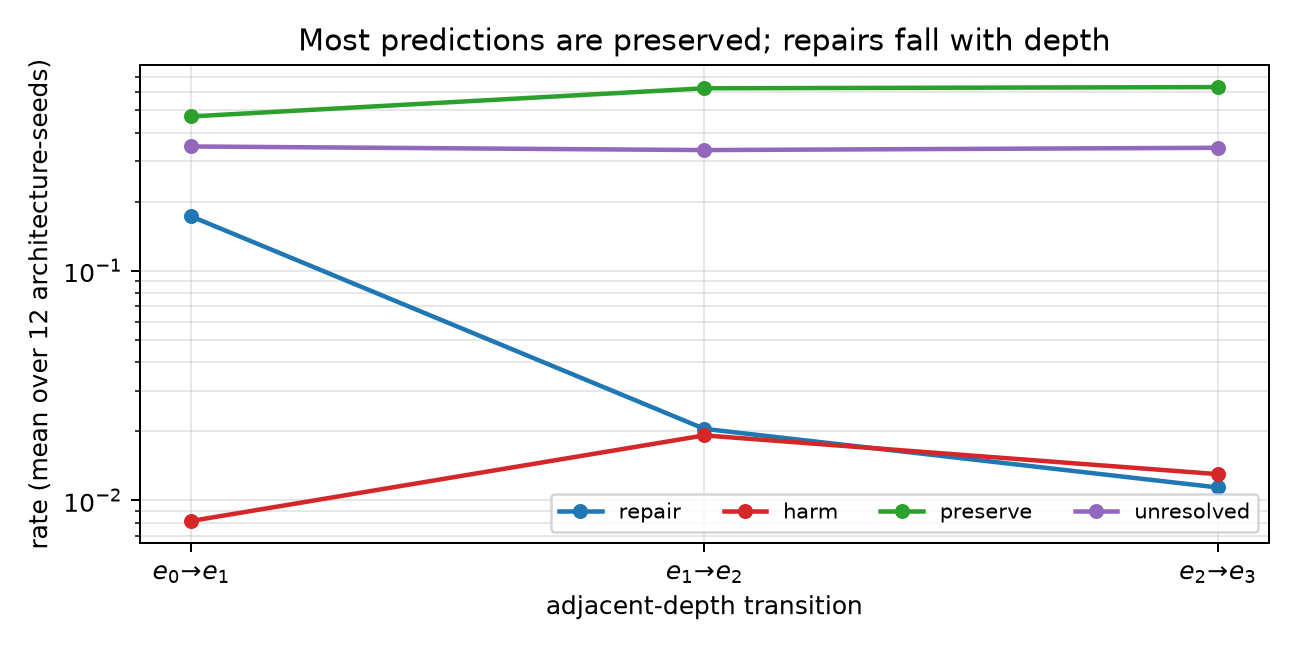
\includegraphics[width=\columnwidth]{figures/fig_transitions.png}
\caption{Prediction transitions between adjacent depths, averaged over 12 architecture-seeds.}
\label{fig:transitions}
\end{figure} Adjacent-depth transitions explain where the early gain comes from. Repairs concentrate in the first refinement: the mean over 12 architecture-seeds falls from 0.173 at $e_0\!\to\!e_1$ to 0.021 and 0.011 later, while preserved predictions rise from 0.471 to 0.632. Harm stays below 0.02 on average, but Transformer reaches 0.043 at $e_1\!\to\!e_2$, so further refinement is not uniformly safe. Unresolved predictions remain near 0.35 throughout and reach 0.59 on LSTM, the portion of the input that extra computation could in principle fix but does not.

\begin{table}[t]
\centering
\footnotesize
\setlength{\tabcolsep}{1.2pt}
\resizebox{\linewidth}{!}{%
\begin{tabular}{@{}llcccccl@{}}
\toprule
Arch & Seed & f-$e_3$ EM & halt EM & $\Delta$EM & 95\% CI & $N_{\mathrm{cell}}$ & NI \\ \midrule
GRU & $s_0$ & $0.879$ & $0.879$ & $+0.00$ & $[0.00,0.00]$ & 0.266 & \checkmark \\
GRU & $s_1$ & $0.844$ & $0.844$ & $+0.00$ & $[0.00,0.00]$ & 0.268 & \checkmark \\
GRU & $s_2$ & $0.891$ & $0.891$ & $+0.00$ & $[0.00,0.00]$ & 0.267 & \checkmark \\
Vanilla RNN & $s_0$ & $0.434$ & $0.438$ & $+0.39$ & $[0.00,1.17]$ & 0.317 & \checkmark \\
Vanilla RNN & $s_1$ & $0.547$ & $0.551$ & $+0.39$ & $[0.00,1.17]$ & 0.324 & \checkmark \\
Vanilla RNN & $s_2$ & $0.480$ & $0.461$ & $-1.95$ & $[-3.91,-0.39]$ & 0.322 & $\times$ \\
LSTM & $s_0$ & $0.629$ & $0.629$ & $+0.00$ & $[0.00,0.00]$ & 0.302 & \checkmark \\
LSTM & $s_1$ & $0.312$ & $0.312$ & $+0.00$ & $[0.00,0.00]$ & 0.320 & \checkmark \\
LSTM & $s_2$ & $0.328$ & $0.328$ & $+0.00$ & $[0.00,0.00]$ & 0.324 & \checkmark \\
Transformer & $s_0$ & $0.871$ & $0.848$ & $-2.34$ & $[-5.47,0.78]$ & 0.260 & $\ ?$ \\
Transformer & $s_1$ & $0.648$ & $0.703$ & $+5.47$ & $[1.17,10.16]$ & 0.262 & \checkmark \\
Transformer & $s_2$ & $0.855$ & $0.809$ & $-4.69$ & $[-7.81,-1.95]$ & 0.267 & $\times$ \\
\bottomrule
\end{tabular}%
}
\caption{Halting on the 256-sample manifest. $\Delta$EM vs. forced $e_3$; NI by LCB$_{95}\geq-0.5$pp. $N_{\mathrm{cell}}$ is the halt-to-forced-$e_3$ call ratio. $\times$: significant loss; $?$: inconclusive. Nine non-inferior, two negative, one inconclusive.}
\label{tab:halt12}
\end{table} Table~\ref{tab:halt12} is the primary accuracy--compute result on the shared 256-sample manifest. The rule is non-inferior or better on 9 of 12 architecture-seeds, significantly worse on two (Vanilla RNN $s_2$: $-1.95$pp, 95\% CI $[-3.91,-0.39]$; Transformer $s_2$: $-4.69$pp, $[-7.81,-1.95]$), and inconclusive on one (Transformer $s_0$: $-2.34$pp, $[-5.47,0.78]$). The $N_{\mathrm{cell}}$ ratio is 0.260--0.324, a 68--74\% reduction in executed decoder and refinement calls, but this does not mean every seed can halt without loss. The rule is safe where the forced-depth curve saturates after $e_1$ and harmful where later depths still help. Non-inferiority is decided by the preregistered bound LCB$_{95}\geq-0.5$pp, not by point estimates.

The call reduction is verified at execution level. Across GRU, Vanilla RNN, and LSTM, 12 settings under forced $e_0$, forced $e_1$, forced $e_3$, and the threshold rule match the reference decoder exactly ($12/12$), and the forward-hook row counts satisfy both identities in all 24 checks. Under forced $e_0$ the instrumented decoder triggers zero refinement calls on all 52{,}458 generated tokens. \begin{table}[t]
\centering
\begin{tabular}{lcccc}
\toprule
Model & $b{=}1$ & $b{=}4$ & $b{=}8$ & $b{=}32$ \\
\midrule
GRU & 0.439 & 0.440 & 0.484 & 0.577 \\
Vanilla RNN & 0.452 & 0.468 & 0.555 & 0.640 \\
LSTM & 0.430 & 0.471 & 0.538 & 0.611 \\
\bottomrule
\end{tabular}
\caption{Halt/forced-$e_3$ median wall-clock ratio of the active-subset executor, two CPU threads, 2 warmup and 10 interleaved passes; $b{=}1$ uses 16 manifest samples, $b{=}4/8/32$ use 64. The per-sample Transformer executor (0.297) is a separate measurement and is not combined here.}
\label{tab:wall}
\end{table} Timing uses two CPU threads, two warmup and ten interleaved passes, with 16 manifest samples at $b{=}1$ and 64 at $b{=}4/8/32$. The active-subset executor gives halt-to-forced-$e_3$ ratios of 0.430--0.640; at $b{=}32$ the saving is about 36--42\%, because base steps, attention, output projection, gating, and per-step Python work are shared by both arms and are not counted by $N_{\mathrm{cell}}$. A separate per-sample Transformer executor gives 0.297 on the same 16 samples; it is a different measurement protocol and is never combined with the active-subset ratios.

\textbf{Cross-architecture latent state dynamics.} \begin{figure}[t]
\centering
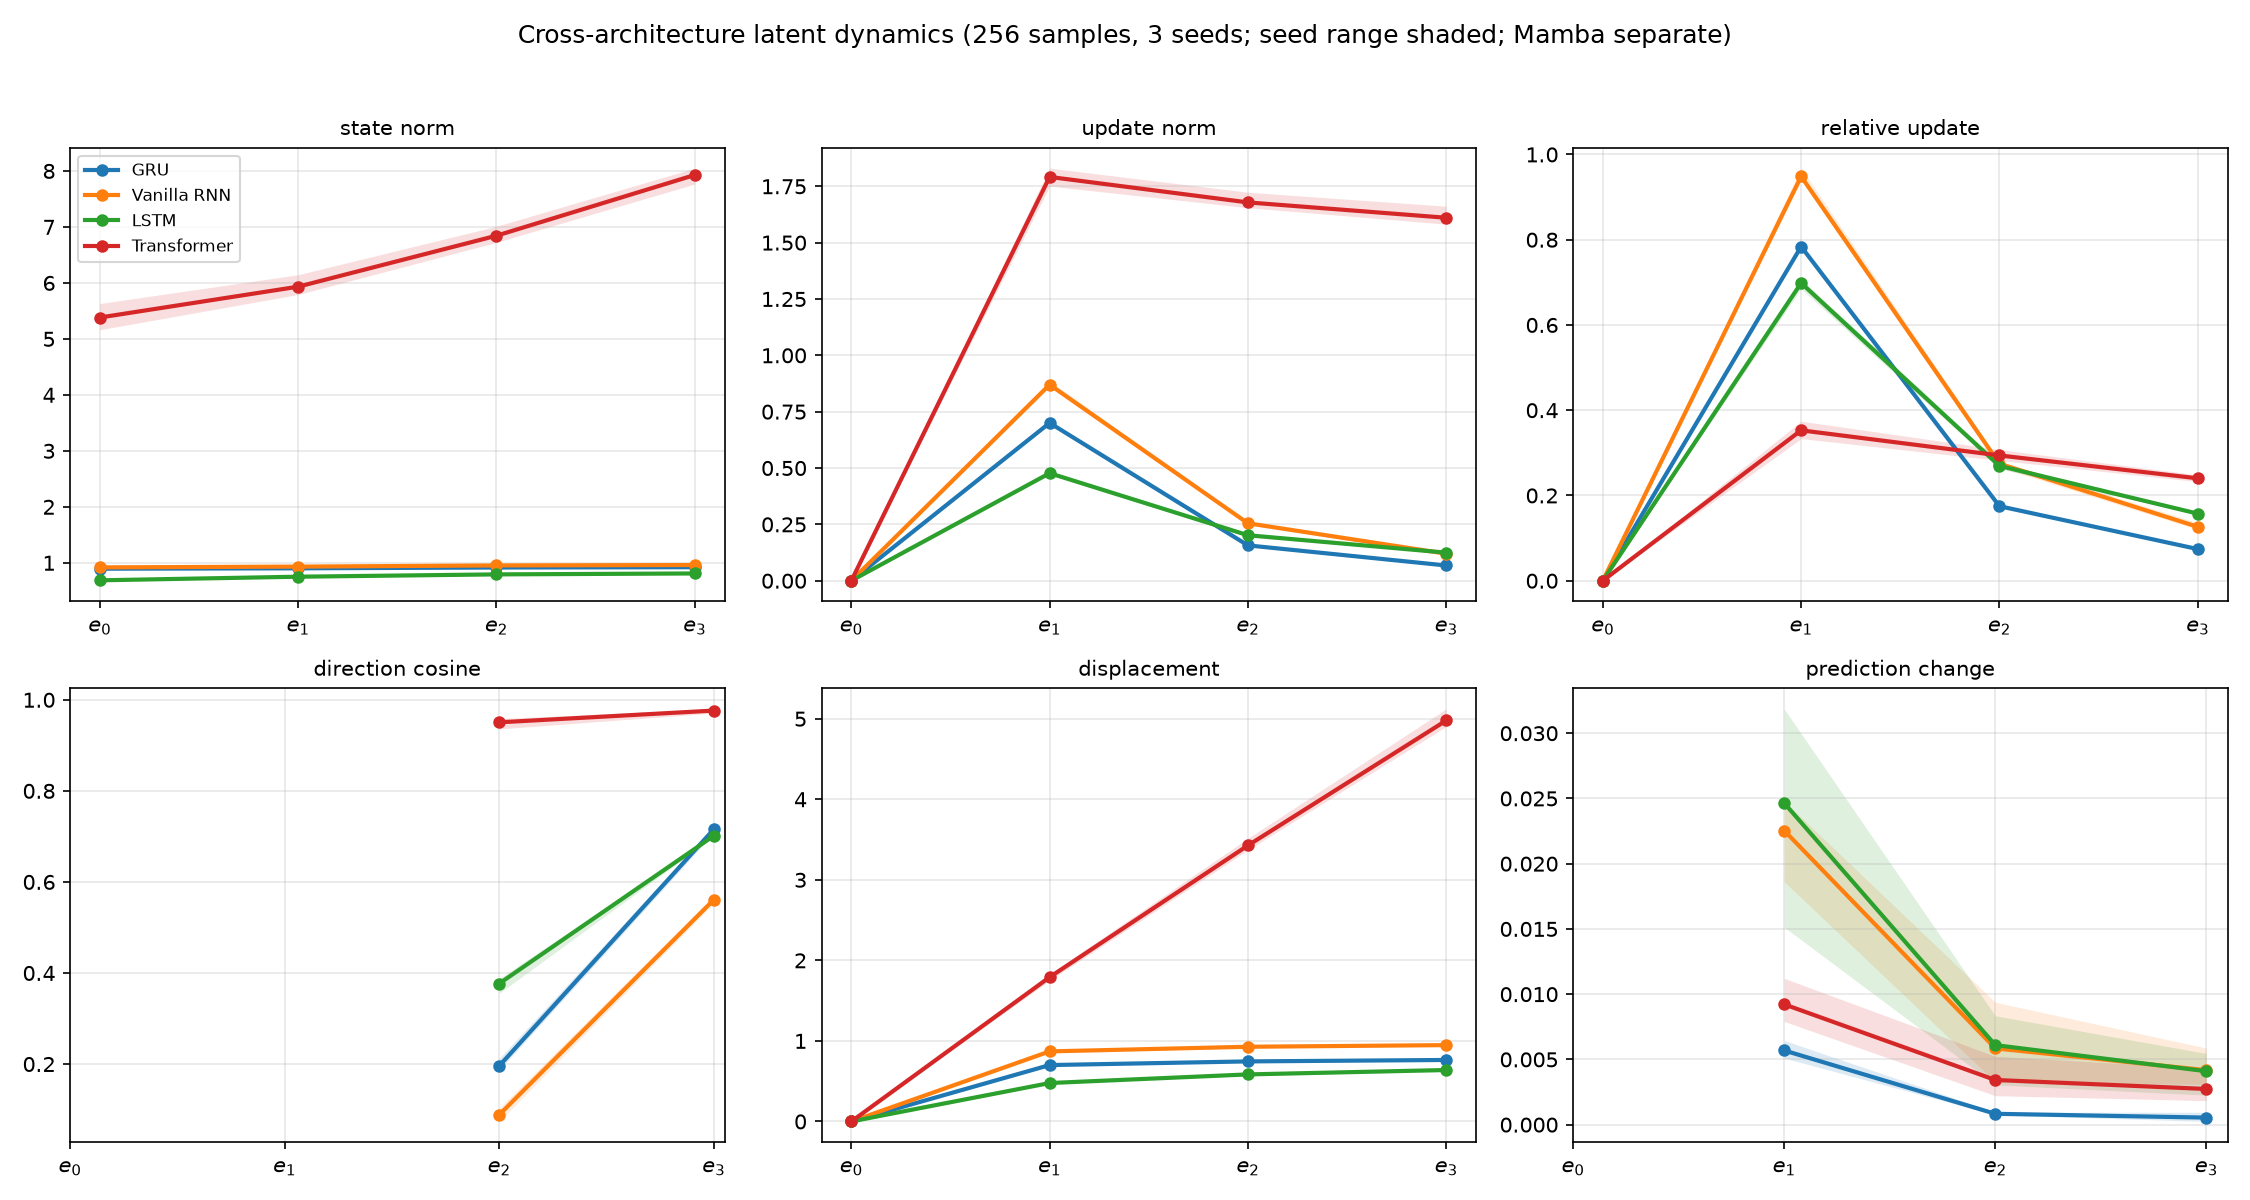
\includegraphics[width=\columnwidth]{figures/crossarch_latent_figure.png}
\caption{Six latent-dynamics metrics across depth; seed ranges shaded.}
\label{fig:latcross}
\end{figure} \begin{table}[t]
\centering
\footnotesize
\resizebox{\linewidth}{!}{%
\begin{tabular}{@{}lcccc@{}}
\toprule
Arch & norm $e_0$ & upd $e_1$ & cos $e_2$ & $\Delta y$ $e_3$ \\ \midrule
GRU & 0.90 $[0.90,0.90]$ & 0.70 $[0.70,0.70]$ & 0.19 $[0.18,0.19]$ & 0.0004 $[0.0002,0.0007]$ \\
Vanilla RNN & 0.92 $[0.92,0.92]$ & 0.89 $[0.88,0.89]$ & 0.09 $[0.09,0.09]$ & 0.0059 $[0.0038,0.0082]$ \\
LSTM & 0.69 $[0.69,0.69]$ & 0.48 $[0.48,0.48]$ & 0.39 $[0.38,0.39]$ & 0.0023 $[0.0014,0.0032]$ \\
Transformer & 5.16 $[5.13,5.20]$ & 1.83 $[1.83,1.84]$ & 0.96 $[0.96,0.96]$ & 0.0020 $[0.0012,0.0030]$ \\
\bottomrule
\end{tabular}%
}
\caption{Seed-0 means with 95\% group-cluster bootstrap intervals (256 samples). Seed ranges across the three seeds are shaded in Figure~\ref{fig:latcross}; norm is $\lVert z_k\rVert/\sqrt d$.}
\label{tab:latstat}
\end{table} Figure~\ref{fig:latcross} and Table~\ref{tab:latstat} summarize six trajectory metrics recorded under free-running greedy decoding on 256 group-balanced samples, with token-level values averaged within each example before a 20{,}000-resample group-cluster bootstrap. Two regimes separate. Bounded gated states (GRU, Vanilla RNN, LSTM hidden state) stay between 0.68 and 0.96 in normalized norm and shrink their updates with depth; the first refinement carries 74--92\% of their total displacement. Unbounded accumulators (LSTM cell state and Transformer) occupy a scale around 5 to 8 and keep changing. LSTM hidden and cell states are reported separately because they behave differently. The sharpest separation is directional: at $e_2$ the bounded group has update cosine 0.07--0.39, whereas Transformer reaches 0.95 with persistently collinear updates and a growing norm. Prediction-change rates decline with depth in every architecture. These are within-model descriptors, not cross-architecture rankings; absolute state norms are not comparable across models, attention type and parameter count co-vary, and the single-seed Mamba-1-Tiny probe is excluded from the four-architecture statistics: its 256-sample group-balanced re-evaluation gives $e_3=0.246$ below the 0.30 gate, and its 64-sample latent trace is descriptive only.

\textbf{Evolutionary step-size control and transfer.} \begin{table}[t]
\centering
\footnotesize
\begin{tabular}{@{}lcccc@{}}
\toprule
Algorithm & Mean (pp) & Median (pp) & Std (pp) & Win \\ \midrule
RS & $+0.64$ & $+0.52$ & 0.63 & 67\% \\
GA & $+0.81$ & $+0.52$ & 0.64 & 89\% \\
MGA & $+0.46$ & $+0.52$ & 0.17 & 89\% \\
DE & $+0.81$ & $+0.52$ & 0.53 & 89\% \\
sepCMA & $+0.41$ & $+0.52$ & 0.35 & 67\% \\
\bottomrule
\end{tabular}
\caption{All five optimizers in the 45-search study (3 model seeds $\times$ 5 algorithms $\times$ 3 optimizer seeds, 336 evaluations each). Gains are in pp over the $\alpha\equiv1$ baseline on the 192-example inner subset; one example equals $0.52$pp. MGA is reported as a separate algorithm.}
\label{tab:opt5}
\end{table} \begin{figure}[t]
\centering
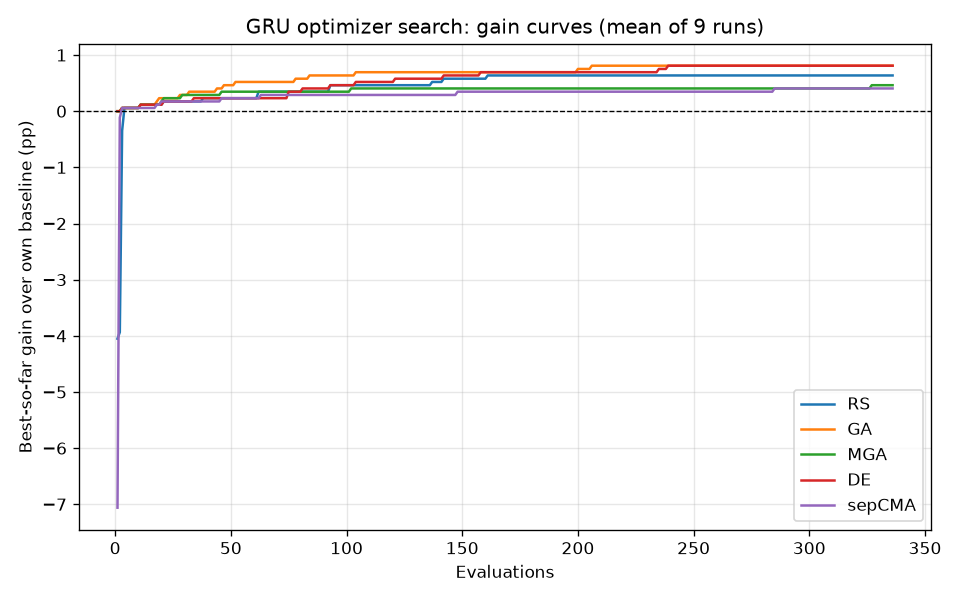
\includegraphics[width=\columnwidth]{figures/optimizer_curves.png}
\caption{Best-so-far gain over each run's own baseline (means of nine runs).}
\label{fig:optcurves}
\end{figure} Table~\ref{tab:opt5} aggregates all 45 searches: 3 model seeds $\times$ 5 algorithms $\times$ 3 optimizer seeds, with 336 evaluations per run. The five optimizers, RS, GA, MGA, DE, and sep-CMA-ES, have the same median gain of $+0.52$pp, exactly one of the 192 inner-subset examples; GA and DE average $+0.81$pp, MGA $+0.46$pp, RS $+0.64$pp, and sep-CMA-ES $+0.41$pp, with win rates of 67--89\%. Baseline EM varies by 2.4pp across model seeds, several times the search effect, and the single $+2.08$pp run is an outlier. Random search is competitive and no optimizer wins consistently; three optimizer seeds do not support an algorithm ranking. The 192-example subset quantizes any gain to roughly 0.52pp, so the resolution limits what can be concluded. Figure~\ref{fig:optcurves} shows each run's best-so-far gain over its own baseline.

\begin{table}[t]
\centering
\footnotesize
\begin{tabular}{@{}llccl@{}}
\toprule
Seed & Best & Outer $\Delta$EM & 95\% CI (pp) & NI \\ \midrule
$s_0$ & DE & $+0.000$ & $[-0.519,+0.527]$ & $\times$ \\
$s_1$ & GA & $-0.469$ & $[-1.357,+0.000]$ & $\times$ \\
$s_2$ & DE & $+0.000$ & $[-0.469,+0.538]$ & \checkmark \\
\bottomrule
\end{tabular}
\caption{Outer-fold confirmation of the three GRU step-size policies ($n=640$ per seed). Only seed 2 meets the non-inferiority bound; seed 0 misses it by 0.019pp (LCB $-0.519$pp).}
\label{tab:alpha_confirm}
\end{table} Selecting a policy on the inner subset and freezing it before outer evaluation gives the confirmation in Table~\ref{tab:alpha_confirm}. Only seed 2 meets the non-inferiority bound on the 640-sample outer fold; seed 0 misses it by 0.019pp (LCB $-0.519$pp) and seed 1 clearly fails. Inner-subset gains therefore do not become reliable outer gains. \begin{table}[t]
\centering
\footnotesize
\setlength{\tabcolsep}{2pt}
\begin{tabular}{@{}lccl@{}}
\toprule
Target & Seed & $\Delta$ (pp) & 95\% CI / verdict \\
\midrule
Vanilla RNN & 0 & $-0.39$ & $[-1.17,0.00]$ inconclusive \\
Vanilla RNN & 1 & $+1.17$ & $[-0.39,3.12]$ non-inferior \\
Vanilla RNN & 2 & $+0.39$ & $[0.00,1.17]$ non-inferior \\
LSTM & 0 & $-0.78$ & $[-1.95,0.00]$ inconclusive \\
LSTM & 1 & $+0.78$ & $[-0.78,2.34]$ inconclusive \\
LSTM & 2 & $-0.39$ & $[-1.17,0.00]$ inconclusive \\
Transformer & 0 & $+2.34$ & $[0.00,4.69]$ non-inferior \\
Transformer & 1 & $+3.52$ & $[0.39,6.64]$ non-inferior \\
Transformer & 2 & $-0.39$ & $[-2.73,1.95]$ inconclusive \\
\bottomrule
\end{tabular}
\caption{Frozen GRU-s0 alpha policy: per-seed EM difference vs.\ forced $e_3$.}
\label{tab:trans}
\end{table} Applying the policy frozen from GRU seed 0, the GA policy selected on that seed, without any target-architecture search to Vanilla RNN, LSTM, and Transformer gives the nine per-seed results in Table~\ref{tab:trans}: four non-inferior, five inconclusive, and no significant loss. The outer confirmation in Table~\ref{tab:alpha_confirm} instead uses each seed's own best inner policy. This is partial transfer under one protocol, not a general cross-architecture capability, and architecture counts are too small for ranking. \begin{table}[t]
\centering
\footnotesize
\setlength{\tabcolsep}{2.5pt}
\resizebox{\linewidth}{!}{%
\begin{tabular}{llccccc}
\toprule
Seed / base & Base EM & Thr.\ EM & $\Delta$EM (pp) & 95\% CI (pp) & ratio & NI \\
\midrule
$s_0$ / $e_3$ & 95.53 & 95.43 & $-0.10$ & $[-0.23, 0.00]$ & 0.2572 & \checkmark \\
$s_1$ / $e_3$ & 97.13 & 97.07 & $-0.07$ & $[-0.17, 0.00]$ & 0.2573 & \checkmark \\
$s_2$ / $e_1$ & 96.77 & 96.97 & $+0.20$ & $[-0.10, +0.51]$ & 0.5182 & \checkmark \\
\bottomrule
\end{tabular}%
}
\caption{\textbf{One-shot confirmation on untouched data.} Official COGS development set ($n{=}3{,}000$; group-cluster paired bootstrap, 20{,}000 resamples), evaluated once with the frozen preregistered threshold and each seed's frozen best fixed depth. The compute ratios match the held-out-fold values (0.2575 / 0.2570 / 0.5212) for seeds 0--1 to the third decimal; seed 2 differs by 0.003 (0.6\% relative), so the executed-call savings transfer across splits to within a fraction of a percent.}
\label{tab:devconfirm}
\end{table} Finally, the frozen threshold rule is evaluated once on the untouched 3{,}000-example COGS development set (Table~\ref{tab:devconfirm}); the executed-call ratios match the held-out values to three decimals on two seeds and differ by 0.003 on the third. Together these results bound the claim: search yields small, resolution-limited gains, and a frozen update policy transfers only on part of the targets.

\section{Conclusion}
\label{sec:conclusion}
The benefit of recursion is not spread evenly across depths. On several seeds the model has already settled after the first refinement, and later steps change little; a causal threshold removes those steps without losing accuracy on most architecture-seeds. Two seeds still lose accuracy under that same fixed threshold, so the saving depends on where each depth curve saturates.

Latent trajectories explain the split. Bounded gated states shrink their updates after the first refinement, whereas unbounded states keep accumulating along a consistent direction. The first-refinement pattern therefore belongs to the bounded regime, not to recursive models in general, and absolute state norms should not be read as a ranking.

Evolutionary search moves the fixed step size only slightly: the median gain is one sample of the 192-example inner subset across 45 searches, and no single optimizer wins consistently. The selected step-size policy passes outer confirmation on one of three seeds, and the same frozen policy is non-inferior on four of nine transfers. These gains do not become reliable cross-architecture improvements; we treat this gap as a substantive limit of the approach.

TRACER is one way to work with recursive computation: trace predictions and states, decide whether to spend another step, and test how far a tuned update travels. More depth is not always more accuracy; knowing when an extra step helps, and whether a control rule still holds on a new model, matters just as much. Taken together, the three lines serve one goal: we trace recursive states to understand when depth helps, halt computation to avoid redundant refinement, and evolve update policies to test how far a policy carries, recording where each rule holds and where it fails.

\section*{Limitations}
Limited computing resources kept the models small and the number of architectures and seeds modest. The primary task is a single semantic parsing dataset (COGS), and the observed patterns should not be assumed to carry to large language models or broader reasoning workloads. Because attention type and parameter count also vary across the four architectures, these comparisons describe behavioral variants under one task rather than controlled ablations of the recurrent cell. Experiments ran on CPU with a fixed two-thread setting, so the wall-clock numbers describe this setting rather than large-scale GPU serving or much deeper recursion; whether the latent dynamics and control rules persist in those regimes remains open.

\bibliography{references}

\end{document}
